\section{Submodule structure}
Being very limited in size, it was quite difficult to come up with a system design. The development processes included several versions of a LiDAR submodule structure and electronics.
The final design is shown in figure \ref{fig:solid_sub}.
In this design we use two MEMS mirrors due to technical reasons. 

\begin{figure}[h]
\center{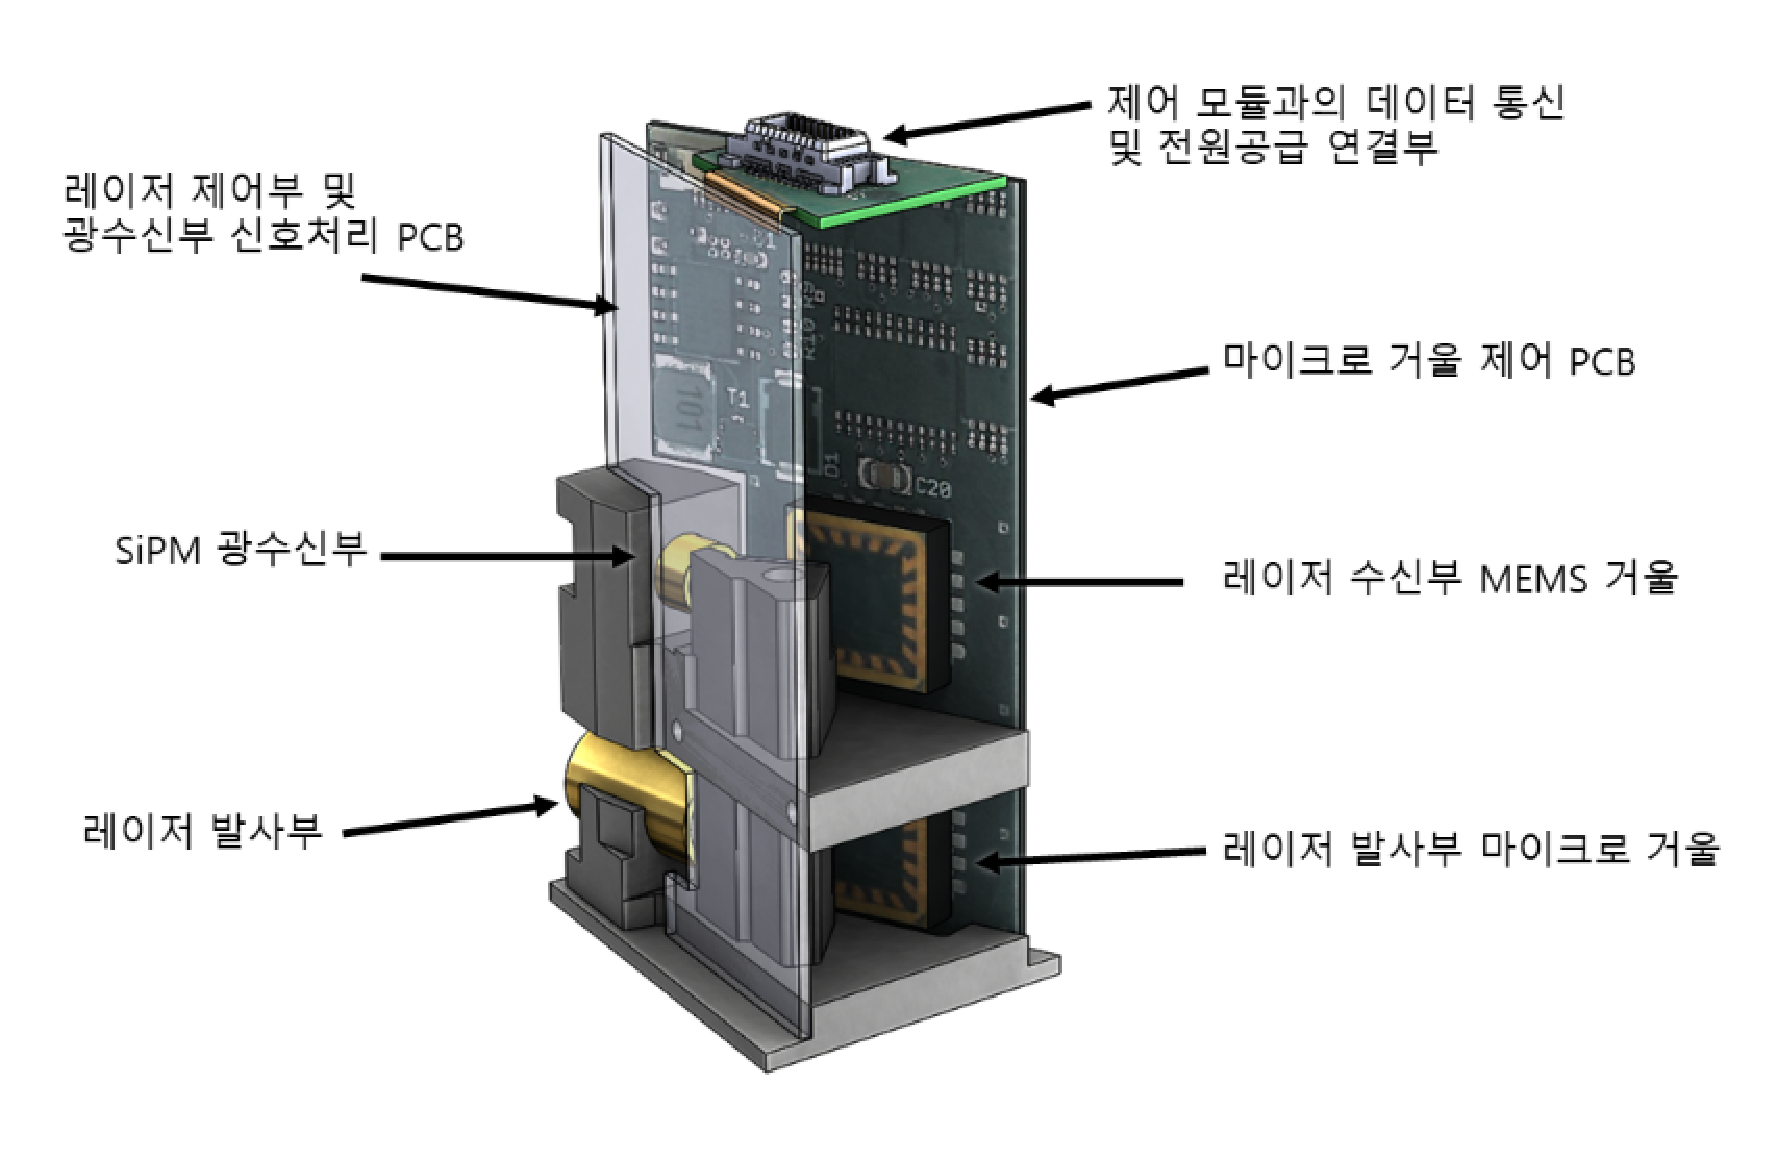
\includegraphics[width=0.8\linewidth]{solidworks_sub}} 
\caption{Final design of the LiDAR submodule.}
\label{fig:solid_sub} 
\end{figure}

The submodule includes the following parts: 
\begin{itemize}
\item Laser module, which consist of laser diode, laser collimator and laser driver electronics.
\item SiPM module, which consist of SiPM collimator, SiPM sensor and its electronics.
\item MEMS module, which consist of MEMS mirror and MEMS driver electronics.
\end{itemize}

The submodel is connected to the control board via a connector located on top.

Laser collimator consists of a tube with an aspheric lens and an laser diode placed in the lens’s focal plane. SiPM has similar structure, but this time a pinhole diaphragm placed in the focal plane to limit detector's FOV. They are separated by a plane to avoid stray light.

The electronics consist of two PCBs. The first PCB focused on beam steering only: MEMS driver board. It has a power (+5V) and control (SPI) input, and it produces a high-voltage (160V) 4-channel signal for MEMS mirror control. The second PCB integrates all functions of LiDAR itself: driving laser diode, generating high voltage for SiPM, readout and amplification of SiPM signal and measuring time delay between outgoing and return impulse. Despite the plentiful functions, we managed to fit all of the components to the single small-dimension device HxDxZ mm.



% Finally, single small-dimension device
